%% abtex2-modelo-trabalho-academico.tex, v-1.9.2 laurocesar
%% Copyright 2012-2014 by abnTeX2 group at http://abntex2.googlecode.com/ 
%%
%% This work may be distributed and/or modified under the
%% conditions of the LaTeX Project Public License, either version 1.3
%% of this license or (at your option) any later version.
%% The latest version of this license is in
%%   http://www.latex-project.org/lppl.txt
%% and version 1.3 or later is part of all distributions of LaTeX
%% version 2005/12/01 or later.
%%
%% This work has the LPPL maintenance status `maintained'.
%% 
%% The Current Maintainer of this work is the abnTeX2 team, led
%% by Lauro César Araujo. Further information are available on 
%% http://abntex2.googlecode.com/
%%
%% This work consists of the files abntex2-modelo-trabalho-academico.tex,
%% abntex2-modelo-include-comandos and abntex2-modelo-references.bib
%%

% ------------------------------------------------------------------------
% ------------------------------------------------------------------------
% abnTeX2: Modelo de Trabalho Academico (tese de doutorado, dissertacao de
% mestrado e trabalhos monograficos em geral) em conformidade com 
% ABNT NBR 14724:2011: Informacao e documentacao - Trabalhos academicos -
% Apresentacao
% ------------------------------------------------------------------------
% ------------------------------------------------------------------------

\documentclass[
    % -- opções da classe memoir --
    12pt,               % tamanho da fonte
    openright,          % capítulos começam em pág ímpar (insere página vazia caso preciso)
   % twoside,            % para impressão em verso e anverso. Oposto a oneside
    oneside,            % para impressão em verso e anverso. Oposto a oneside
    a4paper,            % tamanho do papel. 
    % -- opções da classe abntex2 --
    %chapter=TITLE,     % títulos de capítulos convertidos em letras maiúsculas
    %section=TITLE,     % títulos de seções convertidos em letras maiúsculas
    %subsection=TITLE,  % títulos de subseções convertidos em letras maiúsculas
    %subsubsection=TITLE,% títulos de subsubseções convertidos em letras maiúsculas
    % -- opções do pacote babel --
    english,            % idioma adicional para hifenização
    french,             % idioma adicional para hifenização
    spanish,            % idioma adicional para hifenização
    brazil              % o último idioma é o principal do documento
    ]{abntex2}

% ---
% Pacotes básicos 
% ---
\usepackage{lmodern}            % Usa a fonte Latin Modern          
\usepackage[T1]{fontenc}        % Selecao de codigos de fonte.
\usepackage[utf8]{inputenc}     % Codificacao do documento (conversão automática dos acentos)
\usepackage{lastpage}           % Usado pela Ficha catalográfica
\usepackage{indentfirst}        % Indenta o primeiro parágrafo de cada seção.
\usepackage{color}              % Controle das cores
\usepackage{graphicx}           % Inclusão de gráficos
\usepackage{microtype}          % para melhorias de justificação
% ---
        
% ---
% Pacotes adicionais, usados apenas no âmbito do Modelo Canônico do abnteX2
% ---
\usepackage{lipsum}             % para geração de dummy text
% ---

% ---
% Pacotes de citações
% ---
\usepackage[brazilian,hyperpageref]{backref}     % Paginas com as citações na bibl
\usepackage[alf]{abntex2cite}   % Citações padrão ABNT

% --- 
% CONFIGURAÇÕES DE PACOTES
% --- 

% ---
% Configurações do pacote backref
% Usado sem a opção hyperpageref de backref
\renewcommand{\backrefpagesname}{Citado na(s) página(s):~}
% Texto padrão antes do número das páginas
\renewcommand{\backref}{}
% Define os textos da citação
\renewcommand*{\backrefalt}[4]{
    \ifcase #1 %
        Nenhuma citação no texto.%
    \or
        Citado na página #2.%
    \else
        Citado #1 vezes nas páginas #2.%
    \fi}%
% ---

% ---
% Informações de dados para CAPA e FOLHA DE ROSTO
% ---
\titulo{Título do Trabalho}
\autor{Nome do autor}
\local{Cidade -- UF}
\data{Mês, ano}
\orientador{Nome do orientador}
\coorientador{Nome do coorientador}
\instituicao{%
  Instituto Federal de Educação, Ciência e Tecnologia do Rio Grande do Norte
  \par
  Curso XXXXXXXX
  \par
  Campus XXXXXXXX}
\tipotrabalho{monografia}
% O preambulo deve conter o tipo do trabalho, o objetivo, 
% o nome da instituição e a área de concentração 
\preambulo{Trabalho de Conclusão de Curso apresentado à banca examinadora como requisito parcial a obten\c cão do título de XXXXXXX pelo Instituto Federal de Educa\c cão, Ciência e Tecnologia do Rio Grande do Norte.}
% ---

% ---
% Configurações de aparência do PDF final

% alterando o aspecto da cor azul
\definecolor{blue}{RGB}{41,5,195}

% informações do PDF
\makeatletter
\hypersetup{
        %pagebackref=true,
        pdftitle={\@title}, 
        pdfauthor={\@author},
        pdfsubject={\imprimirpreambulo},
        pdfcreator={LaTeX with abnTeX2},
        pdfkeywords={abnt}{latex}{abntex}{abntex2}{trabalho acadêmico}, 
        colorlinks=true,            % false: boxed links; true: colored links
        linkcolor=blue,             % color of internal links
        citecolor=blue,             % color of links to bibliography
        filecolor=magenta,       % color of file links
        urlcolor=blue,
        bookmarksdepth=4
}
\makeatother
% --- 

% --- 
% Espaçamentos entre linhas e parágrafos 
% --- 

% O tamanho do parágrafo é dado por:
\setlength{\parindent}{1.3cm}

% Controle do espaçamento entre um parágrafo e outro:
\setlength{\parskip}{0.2cm}  % tente também \onelineskip

% ---
% compila o indice
% ---
\makeindex
% ---

% ----
% Início do documento
% ----
\begin{document}

% Retira espaço extra obsoleto entre as frases.
\frenchspacing 

% ----------------------------------------------------------
% ELEMENTOS PRÉ-TEXTUAIS
% ----------------------------------------------------------
% \pretextual

% ---
% Capa
% ---
\imprimircapa
% ---

% ---
% Folha de rosto
% (o * indica que haverá a ficha bibliográfica)
% ---
\imprimirfolhaderosto*
% ---

% ---
% Inserir a ficha bibliografica
% ---

% Isto é um exemplo de Ficha Catalográfica, ou ``Dados internacionais de
% catalogação-na-publicação''. Você pode utilizar este modelo como referência. 
% Porém, provavelmente a biblioteca da sua universidade lhe fornecerá um PDF
% com a ficha catalográfica definitiva após a defesa do trabalho. Quando estiver
% com o documento, salve-o como PDF no diretório do seu projeto e substitua todo
% o conteúdo de implementação deste arquivo pelo comando abaixo:
%
% \begin{fichacatalografica}
%     \includepdf{fig_ficha_catalografica.pdf}
% \end{fichacatalografica}
% ---

% ---
% Inserir folha de aprovação
% ---

% Isto é um exemplo de Folha de aprovação, elemento obrigatório da NBR
% 14724/2011 (seção 4.2.1.3). Você pode utilizar este modelo até a aprovação
% do trabalho. Após isso, substitua todo o conteúdo deste arquivo por uma
% imagem da página assinada pela banca com o comando abaixo:
%
% \includepdf{folhadeaprovacao_final.pdf}
%

\newpage
% ---
% Dedicatória
% ---
\begin{dedicatoria}
   \vspace*{\fill}
   \centering
   \noindent
   \textit{Texto de dedicatória.} \vspace*{\fill}   
\end{dedicatoria}
% ---

% ---
% Agradecimentos
% ---
\begin{agradecimentos}

Texto de agradecimentos.

\end{agradecimentos}
% ---

% ---
% Epígrafe
% ---
\begin{epigrafe}
    \vspace*{\fill}
    \begin{flushright}
        \textit{ ``Texto de epígrafe.'' \\
        (Autor)}
    \end{flushright}
\end{epigrafe}
% ---

% ---
% RESUMOS
% ---

% resumo em português
\setlength{\absparsep}{18pt} % ajusta o espaçamento dos parágrafos do resumo
\begin{resumo}

 Texto do resumo.
 
 \textbf{Palavras-chaves}: palavra 1. palavra 2. palavra 3.
\end{resumo}

% resumo em inglês
\begin{resumo}[Abstract]
 \begin{otherlanguage*}{english}
  
  Abstract text.

   \vspace{\onelineskip}
 
   \noindent 
   \textbf{Key-words}: word 1. word 2. word 3.
 \end{otherlanguage*}
\end{resumo}
% ---

% ---
% inserir lista de ilustrações
% ---
\pdfbookmark[0]{\listfigurename}{lof}
\listoffigures*
\cleardoublepage
% ---

% ---
% inserir lista de tabelas
% ---
\pdfbookmark[0]{\listtablename}{lot}
\listoftables*
\cleardoublepage
% ---

% ---
% inserir lista de abreviaturas e siglas
% ---
\begin{siglas}
  \item[IFRN] Instituto Federal de Educa\c cão, Ciência e Tecnologia do Rio Grande do Norte
\end{siglas}
% ---

% ---
% inserir lista de símbolos
% ---
%\begin{simbolos}
 % \item[$ \Gamma $] Letra grega Gama
 % \item[$ \Lambda $] Lambda
 % \item[$ \zeta $] Letra grega minúscula zeta
 % \item[$ \in $] Pertence
% \end{simbolos}
% ---

% ---
% inserir o sumario
% ---
\pdfbookmark[0]{\contentsname}{toc}
\tableofcontents*
\cleardoublepage
% ---



% ----------------------------------------------------------
% ELEMENTOS TEXTUAIS
% ----------------------------------------------------------
\textual

% ----------------------------------------------------------
% Introdução (exemplo de capítulo sem numeração, mas presente no Sumário)
% ----------------------------------------------------------
\chapter[Introdução]{Introdução}
% ----------------------------------------------------------

\section{Problemática}

\section{Objetivos}

\subsection{Objetivos específicos}

\section{Organização do documento}

% ----------------------------------------------------------
% PARTE
% ----------------------------------------------------------
%\part{Preparação da pesquisa}
% ----------------------------------------------------------

% ----------------------------------------------------------
% PARTE
% ----------------------------------------------------------
%\part{Referenciais teóricos}
% ----------------------------------------------------------

% ---
% Capitulo de revisão de literatura
% ---
\chapter{Desenvolvimento}
% ---
\section{Fundamentação teórica}

\section{Trabalhos relacionados}

\section{Materiais e métodos}

% ---
\chapter{Resultados}
% ---


% ----------------------------------------------------------
% Finaliza a parte no bookmark do PDF
% para que se inicie o bookmark na raiz
% e adiciona espaço de parte no Sumário
% ----------------------------------------------------------
%\phantompart

% ---
% Conclusão (outro exemplo de capítulo sem numeração e presente no sumário)
% ---
\chapter[Conclusão]{Conclusão}
% ---

% ----------------------------------------------------------
% ELEMENTOS PÓS-TEXTUAIS
% ----------------------------------------------------------
\postextual
% ----------------------------------------------------------

% ----------------------------------------------------------
% Referências bibliográficas
% ----------------------------------------------------------
\bibliography{referencias}

% ----------------------------------------------------------
% Glossário
% ----------------------------------------------------------
%
% Consulte o manual da classe abntex2 para orientações sobre o glossário.
%
%\glossary

% ----------------------------------------------------------
% Apêndices
% ----------------------------------------------------------

% ---
% Inicia os apêndices
% ---
\begin{apendicesenv}

% Imprime uma página indicando o início dos apêndices
\partapendices

% ----------------------------------------------------------
\chapter{Título}
% ----------------------------------------------------------

Texto do apêndice.

% ----------------------------------------------------------
\chapter{Título}
% ----------------------------------------------------------

Texto do apêndice.

\end{apendicesenv}
% ---


% ----------------------------------------------------------
% Anexos
% ----------------------------------------------------------

% ---
% Inicia os anexos
% ---
\begin{anexosenv}

% Imprime uma página indicando o início dos anexos
\partanexos

% ---
\chapter{Título}
% ---

Texto do anexo.

% ---
\chapter{Títudo}
% ---

Texto do anexo.

% ---
\chapter{Comandos em \LaTeX}
% ---

\textbf{Exemplo de texto em negrito.}

\textit{Exemplo de texto em itálico.}

\underline{Exemplo de texto sublinhado.}

Exemplo de nota de rodapé\footnote{Descri\c cão da nota de rodapé.}.

Importando a Figura \ref{fig:imagem}.

\begin{figure}[htb]
   \centering
   \caption{Título da imagem}
   \label{fig:imagem}
   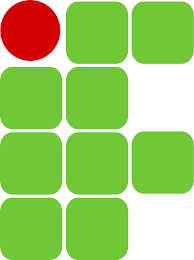
\includegraphics[scale=0.5]{imagens/if}
   \legend{Fonte: XXXXX}
\end{figure}

Construindo a Tabela \ref{tab:tabela}.

\begin{table}[htb]
\center
\footnotesize
\caption{Título da tabela}
\label{tab:tabela}
\begin{tabular} {|c|c|c|c|} % para definir o tamanho usar p{1.4cm}, por exemplo.
  \hline
   \textbf{A} & \textbf{B}  & \textbf{C}  & \textbf{D}  \\
    \hline \hline
    	A1 & B1 & C1& D1\\
   \hline
       	A2 & B2 & C2 & D2\\
   \hline
    	A3 & B3 & C3 & D3\\
   \hline
\end{tabular}
   \legend{Fonte: XXXXX}
\end{table}

Exemplos de cita\c cão: 

\cite[p. 10]{author2020}; ou 

\citeonline[p. 14]{author2020}.

\begin{citacao}
No caso da cita\c cão possuir mais de três linhas, podemos lan\c car mão de um bloco de texto \cite[p. 44]{author2020}.
\end{citacao}

\end{anexosenv}

%---------------------------------------------------------------------
% INDICE REMISSIVO
%---------------------------------------------------------------------
%\phantompart
\printindex
%---------------------------------------------------------------------

\end{document}